\documentclass[1p]{elsarticle_modified}
%\bibliographystyle{elsarticle-num}

%\usepackage[colorlinks]{hyperref}
%\usepackage{abbrmath_seonhwa} %\Abb, \Ascr, \Acal ,\Abf, \Afrak
\usepackage{amsfonts}
\usepackage{amssymb}
\usepackage{amsmath}
\usepackage{amsthm}
\usepackage{scalefnt}
\usepackage{amsbsy}
\usepackage{kotex}
\usepackage{caption}
\usepackage{subfig}
\usepackage{color}
\usepackage{graphicx}
\usepackage{xcolor} %% white, black, red, green, blue, cyan, magenta, yellow
\usepackage{float}
\usepackage{setspace}
\usepackage{hyperref}

\usepackage{tikz}
\usetikzlibrary{arrows}

\usepackage{multirow}
\usepackage{array} % fixed length table
\usepackage{hhline}

%%%%%%%%%%%%%%%%%%%%%
\makeatletter
\renewcommand*\env@matrix[1][\arraystretch]{%
	\edef\arraystretch{#1}%
	\hskip -\arraycolsep
	\let\@ifnextchar\new@ifnextchar
	\array{*\c@MaxMatrixCols c}}
\makeatother %https://tex.stackexchange.com/questions/14071/how-can-i-increase-the-line-spacing-in-a-matrix
%%%%%%%%%%%%%%%

\usepackage[normalem]{ulem}

\newcommand{\msout}[1]{\ifmmode\text{\sout{\ensuremath{#1}}}\else\sout{#1}\fi}
%SOURCE: \msout is \stkout macro in https://tex.stackexchange.com/questions/20609/strikeout-in-math-mode

\newcommand{\cancel}[1]{
	\ifmmode
	{\color{red}\msout{#1}}
	\else
	{\color{red}\sout{#1}}
	\fi
}

\newcommand{\add}[1]{
	{\color{blue}\uwave{#1}}
}

\newcommand{\replace}[2]{
	\ifmmode
	{\color{red}\msout{#1}}{\color{blue}\uwave{#2}}
	\else
	{\color{red}\sout{#1}}{\color{blue}\uwave{#2}}
	\fi
}

\newcommand{\Sol}{\mathcal{S}} %segment
\newcommand{\D}{D} %diagram
\newcommand{\A}{\mathcal{A}} %arc


%%%%%%%%%%%%%%%%%%%%%%%%%%%%%5 test

\def\sl{\operatorname{\textup{SL}}(2,\Cbb)}
\def\psl{\operatorname{\textup{PSL}}(2,\Cbb)}
\def\quan{\mkern 1mu \triangleright \mkern 1mu}

\theoremstyle{definition}
\newtheorem{thm}{Theorem}[section]
\newtheorem{prop}[thm]{Proposition}
\newtheorem{lem}[thm]{Lemma}
\newtheorem{ques}[thm]{Question}
\newtheorem{cor}[thm]{Corollary}
\newtheorem{defn}[thm]{Definition}
\newtheorem{exam}[thm]{Example}
\newtheorem{rmk}[thm]{Remark}
\newtheorem{alg}[thm]{Algorithm}

\newcommand{\I}{\sqrt{-1}}
\begin{document}

%\begin{frontmatter}
%
%\title{Boundary parabolic representations of knots up to 8 crossings}
%
%%% Group authors per affiliation:
%\author{Yunhi Cho} 
%\address{Department of Mathematics, University of Seoul, Seoul, Korea}
%\ead{yhcho@uos.ac.kr}
%
%
%\author{Seonhwa Kim} %\fnref{s_kim}}
%\address{Center for Geometry and Physics, Institute for Basic Science, Pohang, 37673, Korea}
%\ead{ryeona17@ibs.re.kr}
%
%\author{Hyuk Kim}
%\address{Department of Mathematical Sciences, Seoul National University, Seoul 08826, Korea}
%\ead{hyukkim@snu.ac.kr}
%
%\author{Seokbeom Yoon}
%\address{Department of Mathematical Sciences, Seoul National University, Seoul, 08826,  Korea}
%\ead{sbyoon15@snu.ac.kr}
%
%\begin{abstract}
%We find all boundary parabolic representation of knots up to 8 crossings.
%
%\end{abstract}
%\begin{keyword}
%    \MSC[2010] 57M25 
%\end{keyword}
%
%\end{frontmatter}

%\linenumbers
%\tableofcontents
%
\newcommand\colored[1]{\textcolor{white}{\rule[-0.35ex]{0.8em}{1.4ex}}\kern-0.8em\color{red} #1}%
%\newcommand\colored[1]{\textcolor{white}{ #1}\kern-2.17ex	\textcolor{white}{ #1}\kern-1.81ex	\textcolor{white}{ #1}\kern-2.15ex\color{red}#1	}

{\Large $\underline{12n_{0067}~(K12n_{0067})}$}

\setlength{\tabcolsep}{10pt}
\renewcommand{\arraystretch}{1.6}
\vspace{1cm}\begin{tabular}{m{100pt}>{\centering\arraybackslash}m{274pt}}
\multirow{5}{120pt}{
	\centering
	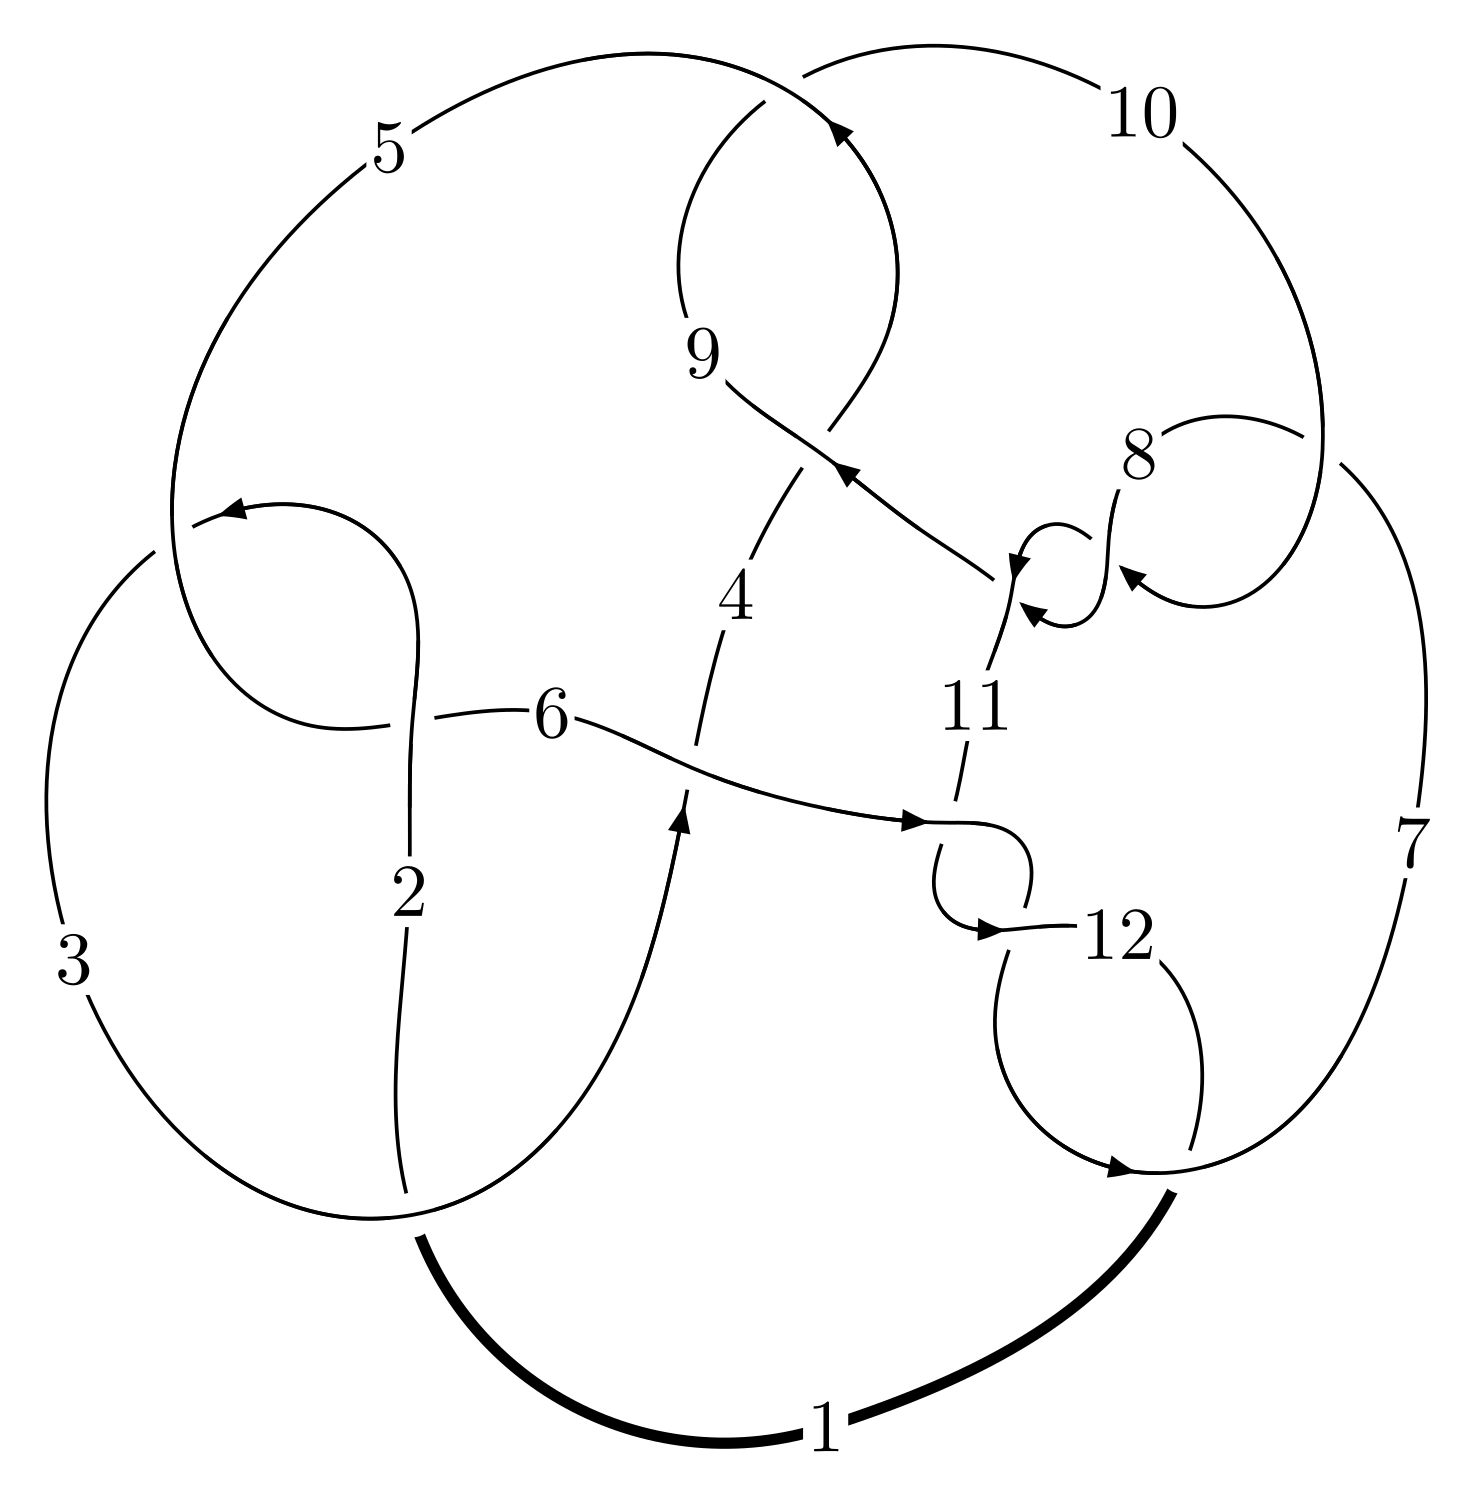
\includegraphics[width=112pt]{../../../GIT/diagram.site/Diagrams/png/2156_12n_0067.png}\\
\ \ \ A knot diagram\footnotemark}&
\allowdisplaybreaks
\textbf{Linearized knot diagam} \\
\cline{2-2}
 &
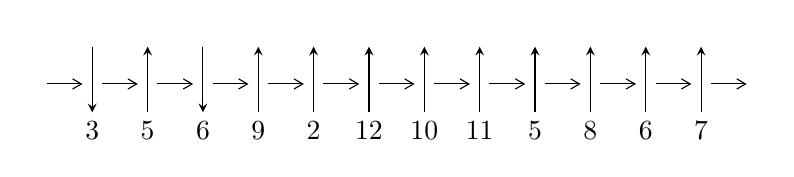
\begin{tikzpicture}[x=20pt, y=17pt]
	% nodes
	\node (C0) at (0, 0) {};
	\node (C1) at (1, 0) {};
	\node (C1U) at (1, +1) {};
	\node (C1D) at (1, -1) {3};

	\node (C2) at (2, 0) {};
	\node (C2U) at (2, +1) {};
	\node (C2D) at (2, -1) {5};

	\node (C3) at (3, 0) {};
	\node (C3U) at (3, +1) {};
	\node (C3D) at (3, -1) {6};

	\node (C4) at (4, 0) {};
	\node (C4U) at (4, +1) {};
	\node (C4D) at (4, -1) {9};

	\node (C5) at (5, 0) {};
	\node (C5U) at (5, +1) {};
	\node (C5D) at (5, -1) {2};

	\node (C6) at (6, 0) {};
	\node (C6U) at (6, +1) {};
	\node (C6D) at (6, -1) {12};

	\node (C7) at (7, 0) {};
	\node (C7U) at (7, +1) {};
	\node (C7D) at (7, -1) {10};

	\node (C8) at (8, 0) {};
	\node (C8U) at (8, +1) {};
	\node (C8D) at (8, -1) {11};

	\node (C9) at (9, 0) {};
	\node (C9U) at (9, +1) {};
	\node (C9D) at (9, -1) {5};

	\node (C10) at (10, 0) {};
	\node (C10U) at (10, +1) {};
	\node (C10D) at (10, -1) {8};

	\node (C11) at (11, 0) {};
	\node (C11U) at (11, +1) {};
	\node (C11D) at (11, -1) {6};

	\node (C12) at (12, 0) {};
	\node (C12U) at (12, +1) {};
	\node (C12D) at (12, -1) {7};
	\node (C13) at (13, 0) {};

	% arrows
	\draw[->,>={angle 60}]
	(C0) edge (C1) (C1) edge (C2) (C2) edge (C3) (C3) edge (C4) (C4) edge (C5) (C5) edge (C6) (C6) edge (C7) (C7) edge (C8) (C8) edge (C9) (C9) edge (C10) (C10) edge (C11) (C11) edge (C12) (C12) edge (C13) ;	\draw[->,>=stealth]
	(C1U) edge (C1D) (C2D) edge (C2U) (C3U) edge (C3D) (C4D) edge (C4U) (C5D) edge (C5U) (C6D) edge (C6U) (C7D) edge (C7U) (C8D) edge (C8U) (C9D) edge (C9U) (C10D) edge (C10U) (C11D) edge (C11U) (C12D) edge (C12U) ;
	\end{tikzpicture} \\
\hhline{~~} \\& 
\textbf{Solving Sequence} \\ \cline{2-2} 
 &
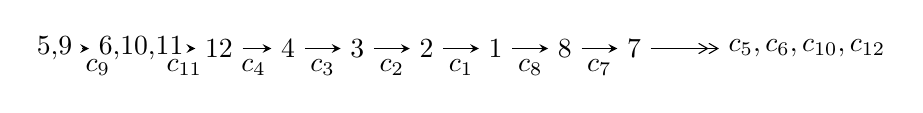
\begin{tikzpicture}[x=25pt, y=7pt]
	% node
	\node (A0) at (-1/8, 0) {5,9};
	\node (A1) at (9/8, 0) {6,10,11};
	\node (A2) at (9/4, 0) {12};
	\node (A3) at (13/4, 0) {4};
	\node (A4) at (17/4, 0) {3};
	\node (A5) at (21/4, 0) {2};
	\node (A6) at (25/4, 0) {1};
	\node (A7) at (29/4, 0) {8};
	\node (A8) at (33/4, 0) {7};
	\node (C1) at (1/2, -1) {$c_{9}$};
	\node (C2) at (7/4, -1) {$c_{11}$};
	\node (C3) at (11/4, -1) {$c_{4}$};
	\node (C4) at (15/4, -1) {$c_{3}$};
	\node (C5) at (19/4, -1) {$c_{2}$};
	\node (C6) at (23/4, -1) {$c_{1}$};
	\node (C7) at (27/4, -1) {$c_{8}$};
	\node (C8) at (31/4, -1) {$c_{7}$};
	\node (A9) at (43/4, 0) {$c_{5},c_{6},c_{10},c_{12}$};

	% edge
	\draw[->,>=stealth]	
	(A0) edge (A1) (A1) edge (A2) (A2) edge (A3) (A3) edge (A4) (A4) edge (A5) (A5) edge (A6) (A6) edge (A7) (A7) edge (A8) ;
	\draw[->>,>={angle 60}]	
	(A8) edge (A9);
\end{tikzpicture} \\ 

\end{tabular} \\

\footnotetext{
The image of knot diagram is generated by the software ``\textbf{Draw programme}" developed by Andrew Bartholomew(\url{http://www.layer8.co.uk/maths/draw/index.htm\#Running-draw}), where we modified some parts for our purpose(\url{https://github.com/CATsTAILs/LinksPainter}).
}\phantom \\ \newline 
\centering \textbf{Ideals for irreducible components\footnotemark of $X_{\text{par}}$} 
 
\begin{align*}
I^u_{1}&=\langle 
5.68457\times10^{17} u^{17}+8.64985\times10^{17} u^{16}+\cdots+1.24822\times10^{20} d+1.55459\times10^{19},\\
\phantom{I^u_{1}}&\phantom{= \langle  }2.99690\times10^{17} u^{17}+2.72458\times10^{17} u^{16}+\cdots+2.49645\times10^{20} c-2.46906\times10^{20},\\
\phantom{I^u_{1}}&\phantom{= \langle  }-4.18893\times10^{15} u^{17}+2.24411\times10^{18} u^{16}+\cdots+1.24822\times10^{20} b-4.97576\times10^{19},\\
\phantom{I^u_{1}}&\phantom{= \langle  }-3.58259\times10^{17} u^{17}-3.47344\times10^{18} u^{16}+\cdots+2.49645\times10^{20} a-2.35898\times10^{20},\\
\phantom{I^u_{1}}&\phantom{= \langle  }u^{18}+3 u^{17}+\cdots+32 u+32\rangle \\
I^u_{2}&=\langle 
-1447 u^9 c-65 u^9+\cdots+7346 c+3206,\;-22391 u^9 c+7563 u^9+\cdots+121770 c-50482,\\
\phantom{I^u_{2}}&\phantom{= \langle  }-378 u^9+149 u^8+\cdots+857 b+1781,\;7265 u^9-363 u^8+\cdots+13712 a-20806,\\
\phantom{I^u_{2}}&\phantom{= \langle  }u^{10}- u^9-7 u^8+8 u^7+13 u^6-14 u^5-2 u^4-2 u^3+13 u^2-12 u+4\rangle \\
\\
I^v_{1}&=\langle 
a,\;d,\;c-1,\;b-1,\;v^2- v+1\rangle \\
I^v_{2}&=\langle 
a,\;d+1,\;c+a,\;b-1,\;v^2- v+1\rangle \\
I^v_{3}&=\langle 
c,\;d+1,\;b,\;a+1,\;v+1\rangle \\
I^v_{4}&=\langle 
c,\;d+1,\;- v^2 b a- v^2 b+a v+c+v,\;b^2 v^2- b v+1\rangle \\
\end{align*}
\raggedright * 5 irreducible components of $\dim_{\mathbb{C}}=0$, with total 43 representations.\\
\raggedright * 1 irreducible components of $\dim_{\mathbb{C}}=1$ \\
\footnotetext{All coefficients of polynomials are rational numbers. But the coefficients are sometimes approximated in decimal forms when there is not enough margin.}
\newpage
\renewcommand{\arraystretch}{1}
\centering \section*{I. $I^u_{1}= \langle 5.68\times10^{17} u^{17}+8.65\times10^{17} u^{16}+\cdots+1.25\times10^{20} d+1.55\times10^{19},\;3.00\times10^{17} u^{17}+2.72\times10^{17} u^{16}+\cdots+2.50\times10^{20} c-2.47\times10^{20},\;-4.19\times10^{15} u^{17}+2.24\times10^{18} u^{16}+\cdots+1.25\times10^{20} b-4.98\times10^{19},\;-3.58\times10^{17} u^{17}-3.47\times10^{18} u^{16}+\cdots+2.50\times10^{20} a-2.36\times10^{20},\;u^{18}+3 u^{17}+\cdots+32 u+32 \rangle$}
\flushleft \textbf{(i) Arc colorings}\\
\begin{tabular}{m{7pt} m{180pt} m{7pt} m{180pt} }
\flushright $a_{5}=$&$\begin{pmatrix}0\\u\end{pmatrix}$ \\
\flushright $a_{9}=$&$\begin{pmatrix}1\\0\end{pmatrix}$ \\
\flushright $a_{6}=$&$\begin{pmatrix}0.00143508 u^{17}+0.0139135 u^{16}+\cdots-0.714624 u+0.944936\\0.0000335592 u^{17}-0.0179784 u^{16}+\cdots+1.37888 u+0.398628\end{pmatrix}$ \\
\flushright $a_{10}=$&$\begin{pmatrix}1\\- u^2\end{pmatrix}$ \\
\flushright $a_{11}=$&$\begin{pmatrix}-0.00120047 u^{17}-0.00109138 u^{16}+\cdots-0.0893825 u+0.989028\\-0.00455413 u^{17}-0.00692973 u^{16}+\cdots-0.245124 u-0.124544\end{pmatrix}$ \\
\flushright $a_{12}=$&$\begin{pmatrix}-0.00490067 u^{17}-0.0153878 u^{16}+\cdots+0.466611 u+1.14967\\0.00513528 u^{17}+0.0282099 u^{16}+\cdots-1.27062 u-0.215706\end{pmatrix}$ \\
\flushright $a_{4}=$&$\begin{pmatrix}- u\\u\end{pmatrix}$ \\
\flushright $a_{3}=$&$\begin{pmatrix}0.000371161 u^{17}+0.0231129 u^{16}+\cdots+0.350709 u-0.584653\\0.0295819 u^{17}+0.0399851 u^{16}+\cdots+2.27781 u+1.67132\end{pmatrix}$ \\
\flushright $a_{2}=$&$\begin{pmatrix}0.000371161 u^{17}+0.0231129 u^{16}+\cdots+0.350709 u-0.584653\\0.0113208 u^{17}+0.00191842 u^{16}+\cdots+1.56195 u+0.967341\end{pmatrix}$ \\
\flushright $a_{1}=$&$\begin{pmatrix}-0.00146864 u^{17}+0.00406488 u^{16}+\cdots-0.664258 u-1.34356\\0.0141649 u^{17}+0.00737088 u^{16}+\cdots+1.60295 u+0.669693\end{pmatrix}$ \\
\flushright $a_{8}=$&$\begin{pmatrix}-0.00120047 u^{17}-0.00109138 u^{16}+\cdots-0.0893825 u+0.989028\\0.00756978 u^{17}+0.0124143 u^{16}+\cdots+0.287029 u+0.204865\end{pmatrix}$ \\
\flushright $a_{7}=$&$\begin{pmatrix}-0.00575459 u^{17}-0.00802111 u^{16}+\cdots-0.334506 u+0.864484\\0.0164592 u^{17}+0.0311513 u^{16}+\cdots+0.356742 u+0.420310\end{pmatrix}$\\&\end{tabular}
\flushleft \textbf{(ii) Obstruction class $= -1$}\\~\\
\flushleft \textbf{(iii) Cusp Shapes $= \frac{1881106086253954753}{31205580083057755580} u^{17}+\frac{5887773742508132609}{62411160166115511160} u^{16}+\cdots+\frac{57261478582730965292}{7801395020764438895} u+\frac{64355080374530213256}{7801395020764438895}$}\\~\\
\newpage\renewcommand{\arraystretch}{1}
\flushleft \textbf{(iv) u-Polynomials at the component}\newline \\
\begin{tabular}{m{50pt}|m{274pt}}
Crossings & \hspace{64pt}u-Polynomials at each crossing \\
\hline $$\begin{aligned}c_{1}\end{aligned}$$&$\begin{aligned}
&u^{18}+5 u^{17}+\cdots-136 u+16
\end{aligned}$\\
\hline $$\begin{aligned}c_{2},c_{5}\end{aligned}$$&$\begin{aligned}
&u^{18}+u^{17}+\cdots-12 u+4
\end{aligned}$\\
\hline $$\begin{aligned}c_{3}\end{aligned}$$&$\begin{aligned}
&u^{18}- u^{17}+\cdots-756 u+1252
\end{aligned}$\\
\hline $$\begin{aligned}c_{4},c_{9}\end{aligned}$$&$\begin{aligned}
&u^{18}+3 u^{17}+\cdots+32 u+32
\end{aligned}$\\
\hline $$\begin{aligned}c_{6},c_{7},c_{8}\\c_{10},c_{11},c_{12}\end{aligned}$$&$\begin{aligned}
&u^{18}+5 u^{17}+\cdots-2 u-1
\end{aligned}$\\
\hline
\end{tabular}\\~\\
\newpage\renewcommand{\arraystretch}{1}
\flushleft \textbf{(v) Riley Polynomials at the component}\newline \\
\begin{tabular}{m{50pt}|m{274pt}}
Crossings & \hspace{64pt}Riley Polynomials at each crossing \\
\hline $$\begin{aligned}c_{1}\end{aligned}$$&$\begin{aligned}
&y^{18}+17 y^{17}+\cdots-38944 y+256
\end{aligned}$\\
\hline $$\begin{aligned}c_{2},c_{5}\end{aligned}$$&$\begin{aligned}
&y^{18}+5 y^{17}+\cdots-136 y+16
\end{aligned}$\\
\hline $$\begin{aligned}c_{3}\end{aligned}$$&$\begin{aligned}
&y^{18}+29 y^{17}+\cdots-3653960 y+1567504
\end{aligned}$\\
\hline $$\begin{aligned}c_{4},c_{9}\end{aligned}$$&$\begin{aligned}
&y^{18}-15 y^{17}+\cdots-2048 y+1024
\end{aligned}$\\
\hline $$\begin{aligned}c_{6},c_{7},c_{8}\\c_{10},c_{11},c_{12}\end{aligned}$$&$\begin{aligned}
&y^{18}-29 y^{17}+\cdots-26 y+1
\end{aligned}$\\
\hline
\end{tabular}\\~\\
\newpage\flushleft \textbf{(vi) Complex Volumes and Cusp Shapes}
$$\begin{array}{c|c|c}  
\text{Solutions to }I^u_{1}& \I (\text{vol} + \sqrt{-1}CS) & \text{Cusp shape}\\
 \hline 
\begin{aligned}
u &= -1.078440 + 0.216619 I \\
a &= \phantom{-}0.253388 - 1.028300 I \\
b &= -0.71841 + 2.42684 I \\
c &= \phantom{-}0.492205 - 0.156710 I \\
d &= -0.844681 - 0.587317 I\end{aligned}
 & \phantom{-}3.61986 + 3.92600 I & \phantom{-}13.3379 - 5.7849 I \\ \hline\begin{aligned}
u &= -1.078440 - 0.216619 I \\
a &= \phantom{-}0.253388 + 1.028300 I \\
b &= -0.71841 - 2.42684 I \\
c &= \phantom{-}0.492205 + 0.156710 I \\
d &= -0.844681 + 0.587317 I\end{aligned}
 & \phantom{-}3.61986 - 3.92600 I & \phantom{-}13.3379 + 5.7849 I \\ \hline\begin{aligned}
u &= \phantom{-}0.709201 + 0.274453 I \\
a &= -0.01264 + 1.59035 I \\
b &= \phantom{-}0.27741 - 3.38402 I \\
c &= \phantom{-}0.515734 + 0.082365 I \\
d &= -0.890761 + 0.301961 I\end{aligned}
 & \phantom{-}3.12578 + 1.29944 I & \phantom{-}14.10514 - 0.79844 I \\ \hline\begin{aligned}
u &= \phantom{-}0.709201 - 0.274453 I \\
a &= -0.01264 - 1.59035 I \\
b &= \phantom{-}0.27741 + 3.38402 I \\
c &= \phantom{-}0.515734 - 0.082365 I \\
d &= -0.890761 - 0.301961 I\end{aligned}
 & \phantom{-}3.12578 - 1.29944 I & \phantom{-}14.10514 + 0.79844 I \\ \hline\begin{aligned}
u &= -0.610909 + 0.417338 I \\
a &= \phantom{-}0.428235 + 0.847865 I \\
b &= -0.502581 - 0.271599 I \\
c &= \phantom{-}0.768504 + 0.302779 I \\
d &= -0.126387 + 0.443779 I\end{aligned}
 & -1.20916 - 1.63680 I & \phantom{-}1.95124 + 5.83411 I \\ \hline\begin{aligned}
u &= -0.610909 - 0.417338 I \\
a &= \phantom{-}0.428235 - 0.847865 I \\
b &= -0.502581 + 0.271599 I \\
c &= \phantom{-}0.768504 - 0.302779 I \\
d &= -0.126387 - 0.443779 I\end{aligned}
 & -1.20916 + 1.63680 I & \phantom{-}1.95124 - 5.83411 I\\
 \hline 
 \end{array}$$\newpage$$\begin{array}{c|c|c}  
\text{Solutions to }I^u_{1}& \I (\text{vol} + \sqrt{-1}CS) & \text{Cusp shape}\\
 \hline 
\begin{aligned}
u &= \phantom{-}0.555399\phantom{ +0.000000I} \\
a &= \phantom{-}0.144993\phantom{ +0.000000I} \\
b &= \phantom{-}0.407093\phantom{ +0.000000I} \\
c &= \phantom{-}0.739573\phantom{ +0.000000I} \\
d &= -0.352132\phantom{ +0.000000I}\end{aligned}
 & \phantom{-}0.726383\phantom{ +0.000000I} & \phantom{-}14.1310\phantom{ +0.000000I} \\ \hline\begin{aligned}
u &= -0.072203 + 0.503217 I \\
a &= \phantom{-}2.01283 + 0.53928 I \\
b &= \phantom{-}0.179243 + 0.151857 I \\
c &= \phantom{-}1.330050 + 0.161709 I \\
d &= \phantom{-}0.259101 + 0.090079 I\end{aligned}
 & \phantom{-}0.39079 + 2.25423 I & \phantom{-}1.75748 - 3.62098 I \\ \hline\begin{aligned}
u &= -0.072203 - 0.503217 I \\
a &= \phantom{-}2.01283 - 0.53928 I \\
b &= \phantom{-}0.179243 - 0.151857 I \\
c &= \phantom{-}1.330050 - 0.161709 I \\
d &= \phantom{-}0.259101 - 0.090079 I\end{aligned}
 & \phantom{-}0.39079 - 2.25423 I & \phantom{-}1.75748 + 3.62098 I \\ \hline\begin{aligned}
u &= -1.83506 + 0.34828 I \\
a &= \phantom{-}0.808325 + 0.623484 I \\
b &= -0.014393 - 0.834480 I \\
c &= -1.318640 - 0.296832 I \\
d &= \phantom{-}1.72178 - 0.16248 I\end{aligned}
 & \phantom{-}11.72250 - 5.21750 I & \phantom{-}12.21552 + 2.94469 I \\ \hline\begin{aligned}
u &= -1.83506 - 0.34828 I \\
a &= \phantom{-}0.808325 - 0.623484 I \\
b &= -0.014393 + 0.834480 I \\
c &= -1.318640 + 0.296832 I \\
d &= \phantom{-}1.72178 + 0.16248 I\end{aligned}
 & \phantom{-}11.72250 + 5.21750 I & \phantom{-}12.21552 - 2.94469 I \\ \hline\begin{aligned}
u &= -1.70473 + 1.04671 I \\
a &= -0.230730 + 0.966273 I \\
b &= -0.03020 - 2.29892 I \\
c &= -0.961354 - 0.702659 I \\
d &= \phantom{-}1.67800 - 0.49555 I\end{aligned}
 & -19.5607 - 13.8899 I & \phantom{-}13.2954 + 6.2001 I\\
 \hline 
 \end{array}$$\newpage$$\begin{array}{c|c|c}  
\text{Solutions to }I^u_{1}& \I (\text{vol} + \sqrt{-1}CS) & \text{Cusp shape}\\
 \hline 
\begin{aligned}
u &= -1.70473 - 1.04671 I \\
a &= -0.230730 - 0.966273 I \\
b &= -0.03020 + 2.29892 I \\
c &= -0.961354 + 0.702659 I \\
d &= \phantom{-}1.67800 + 0.49555 I\end{aligned}
 & -19.5607 + 13.8899 I & \phantom{-}13.2954 - 6.2001 I \\ \hline\begin{aligned}
u &= -0.16477 + 2.05598 I \\
a &= \phantom{-}0.905061 - 0.066880 I \\
b &= \phantom{-}0.464341 + 0.377003 I \\
c &= \phantom{-}0.354039 - 0.009486 I \\
d &= -1.82253 - 0.07562 I\end{aligned}
 & \phantom{-}15.4858 + 3.5329 I & \phantom{-}13.90580 - 2.19457 I \\ \hline\begin{aligned}
u &= -0.16477 - 2.05598 I \\
a &= \phantom{-}0.905061 + 0.066880 I \\
b &= \phantom{-}0.464341 - 0.377003 I \\
c &= \phantom{-}0.354039 + 0.009486 I \\
d &= -1.82253 + 0.07562 I\end{aligned}
 & \phantom{-}15.4858 - 3.5329 I & \phantom{-}13.90580 + 2.19457 I \\ \hline\begin{aligned}
u &= \phantom{-}2.12691\phantom{ +0.000000I} \\
a &= \phantom{-}0.609160\phantom{ +0.000000I} \\
b &= \phantom{-}0.619389\phantom{ +0.000000I} \\
c &= -1.17023\phantom{ +0.000000I} \\
d &= \phantom{-}1.85453\phantom{ +0.000000I}\end{aligned}
 & \phantom{-}16.6053\phantom{ +0.000000I} & \phantom{-}15.4680\phantom{ +0.000000I} \\ \hline\begin{aligned}
u &= \phantom{-}1.91575 + 0.96837 I \\
a &= -0.041545 - 0.774296 I \\
b &= \phantom{-}0.33135 + 2.10179 I \\
c &= -0.965214 + 0.561225 I \\
d &= \phantom{-}1.77427 + 0.45020 I\end{aligned}
 & -18.1284 + 6.9769 I & \phantom{-}14.6320 - 1.8700 I \\ \hline\begin{aligned}
u &= \phantom{-}1.91575 - 0.96837 I \\
a &= -0.041545 + 0.774296 I \\
b &= \phantom{-}0.33135 - 2.10179 I \\
c &= -0.965214 - 0.561225 I \\
d &= \phantom{-}1.77427 - 0.45020 I\end{aligned}
 & -18.1284 - 6.9769 I & \phantom{-}14.6320 + 1.8700 I\\
 \hline 
 \end{array}$$\newpage\newpage\renewcommand{\arraystretch}{1}
\centering \section*{II. $I^u_{2}= \langle -1447 c u^{9}-65 u^{9}+\cdots+7346 c+3206,\;-2.24\times10^{4} c u^{9}+7563 u^{9}+\cdots+1.22\times10^{5} c-5.05\times10^{4},\;-378 u^{9}+149 u^{8}+\cdots+857 b+1781,\;7265 u^{9}-363 u^{8}+\cdots+1.37\times10^{4} a-2.08\times10^{4},\;u^{10}- u^9+\cdots-12 u+4 \rangle$}
\flushleft \textbf{(i) Arc colorings}\\
\begin{tabular}{m{7pt} m{180pt} m{7pt} m{180pt} }
\flushright $a_{5}=$&$\begin{pmatrix}0\\u\end{pmatrix}$ \\
\flushright $a_{9}=$&$\begin{pmatrix}1\\0\end{pmatrix}$ \\
\flushright $a_{6}=$&$\begin{pmatrix}-0.529828 u^{9}+0.0264732 u^{8}+\cdots-4.18035 u+1.51736\\0.441074 u^{9}-0.173862 u^{8}+\cdots+4.90898 u-2.07818\end{pmatrix}$ \\
\flushright $a_{10}=$&$\begin{pmatrix}1\\- u^2\end{pmatrix}$ \\
\flushright $a_{11}=$&$\begin{pmatrix}c\\0.422112 c u^{9}+0.0189615 u^{9}+\cdots-2.14294 c-0.935239\end{pmatrix}$ \\
\flushright $a_{12}=$&$\begin{pmatrix}-0.0189615 c u^{9}-0.529828 u^{9}+\cdots+0.935239 c+1.51736\\0.199533 c u^{9}+0.460035 u^{9}+\cdots-0.487748 c-3.01342\end{pmatrix}$ \\
\flushright $a_{4}=$&$\begin{pmatrix}- u\\u\end{pmatrix}$ \\
\flushright $a_{3}=$&$\begin{pmatrix}0.893451 u^{9}-0.113258 u^{8}+\cdots+6.74818 u-3.90621\\-0.258897 u^{9}+0.0170653 u^{8}+\cdots-1.24023 u+1.07730\end{pmatrix}$ \\
\flushright $a_{2}=$&$\begin{pmatrix}0.893451 u^{9}-0.113258 u^{8}+\cdots+6.74818 u-3.90621\\0.381418 u^{9}-0.120916 u^{8}+\cdots+4.54828 u-2.04347\end{pmatrix}$ \\
\flushright $a_{1}=$&$\begin{pmatrix}0.0887544 u^{9}+0.147389 u^{8}+\cdots-0.728632 u+0.560823\\0.145566 u^{9}-0.271004 u^{8}+\cdots+2.43028 u-1.13361\end{pmatrix}$ \\
\flushright $a_{8}=$&$\begin{pmatrix}c\\-0.422112 c u^{9}-0.0189615 u^{9}+\cdots+2.14294 c+0.935239\end{pmatrix}$ \\
\flushright $a_{7}=$&$\begin{pmatrix}0.422112 c u^{9}+0.0189615 u^{9}+\cdots-1.14294 c-0.935239\\-0.387106 c u^{9}-0.218495 u^{9}+\cdots+2.72404 c+1.42299\end{pmatrix}$\\&\end{tabular}
\flushleft \textbf{(ii) Obstruction class $= -1$}\\~\\
\flushleft \textbf{(iii) Cusp Shapes $= \frac{3875}{1714} u^9-\frac{183}{1714} u^8-\frac{26957}{1714} u^7+\frac{2248}{857} u^6+\frac{51811}{1714} u^5+\frac{541}{857} u^4-\frac{185}{857} u^3-\frac{9943}{857} u^2+\frac{27495}{1714} u+\frac{882}{857}$}\\~\\
\newpage\renewcommand{\arraystretch}{1}
\flushleft \textbf{(iv) u-Polynomials at the component}\newline \\
\begin{tabular}{m{50pt}|m{274pt}}
Crossings & \hspace{64pt}u-Polynomials at each crossing \\
\hline $$\begin{aligned}c_{1}\end{aligned}$$&$\begin{aligned}
&(u^{10}+2 u^9+9 u^8+14 u^7+28 u^6+31 u^5+35 u^4+20 u^3+15 u^2+5 u+1)^{2}
\end{aligned}$\\
\hline $$\begin{aligned}c_{2},c_{5}\end{aligned}$$&$\begin{aligned}
&(u^{10}+2 u^9+3 u^8+2 u^7+4 u^6+3 u^5+3 u^4+3 u^2+u+1)^2
\end{aligned}$\\
\hline $$\begin{aligned}c_{3}\end{aligned}$$&$\begin{aligned}
&(u^{10}-2 u^9+\cdots+21 u+17)^{2}
\end{aligned}$\\
\hline $$\begin{aligned}c_{4},c_{9}\end{aligned}$$&$\begin{aligned}
&(u^{10}- u^9-7 u^8+8 u^7+13 u^6-14 u^5-2 u^4-2 u^3+13 u^2-12 u+4)^2
\end{aligned}$\\
\hline $$\begin{aligned}c_{6},c_{7},c_{8}\\c_{10},c_{11},c_{12}\end{aligned}$$&$\begin{aligned}
&u^{20}+3 u^{19}+\cdots-8 u+16
\end{aligned}$\\
\hline
\end{tabular}\\~\\
\newpage\renewcommand{\arraystretch}{1}
\flushleft \textbf{(v) Riley Polynomials at the component}\newline \\
\begin{tabular}{m{50pt}|m{274pt}}
Crossings & \hspace{64pt}Riley Polynomials at each crossing \\
\hline $$\begin{aligned}c_{1}\end{aligned}$$&$\begin{aligned}
&(y^{10}+14 y^9+\cdots+5 y+1)^{2}
\end{aligned}$\\
\hline $$\begin{aligned}c_{2},c_{5}\end{aligned}$$&$\begin{aligned}
&(y^{10}+2 y^9+9 y^8+14 y^7+28 y^6+31 y^5+35 y^4+20 y^3+15 y^2+5 y+1)^{2}
\end{aligned}$\\
\hline $$\begin{aligned}c_{3}\end{aligned}$$&$\begin{aligned}
&(y^{10}+26 y^9+\cdots+2925 y+289)^{2}
\end{aligned}$\\
\hline $$\begin{aligned}c_{4},c_{9}\end{aligned}$$&$\begin{aligned}
&(y^{10}-15 y^9+\cdots-40 y+16)^{2}
\end{aligned}$\\
\hline $$\begin{aligned}c_{6},c_{7},c_{8}\\c_{10},c_{11},c_{12}\end{aligned}$$&$\begin{aligned}
&y^{20}-19 y^{19}+\cdots+1248 y+256
\end{aligned}$\\
\hline
\end{tabular}\\~\\
\newpage\flushleft \textbf{(vi) Complex Volumes and Cusp Shapes}
$$\begin{array}{c|c|c}  
\text{Solutions to }I^u_{2}& \I (\text{vol} + \sqrt{-1}CS) & \text{Cusp shape}\\
 \hline 
\begin{aligned}
u &= -0.620250 + 0.748934 I \\
a &= -0.676664 + 0.412835 I \\
b &= -0.425803 + 0.101141 I \\
c &= \phantom{-}0.448932 - 0.060647 I \\
d &= -1.187590 - 0.295523 I\end{aligned}
 & \phantom{-}4.43566 - 1.46073 I & \phantom{-}14.6593 + 3.2864 I \\ \hline\begin{aligned}
u &= -0.620250 + 0.748934 I \\
a &= -0.676664 + 0.412835 I \\
b &= -0.425803 + 0.101141 I \\
c &= -0.77388 - 2.52919 I \\
d &= \phantom{-}1.110620 - 0.361536 I\end{aligned}
 & \phantom{-}4.43566 - 1.46073 I & \phantom{-}14.6593 + 3.2864 I \\ \hline\begin{aligned}
u &= -0.620250 - 0.748934 I \\
a &= -0.676664 - 0.412835 I \\
b &= -0.425803 - 0.101141 I \\
c &= \phantom{-}0.448932 + 0.060647 I \\
d &= -1.187590 + 0.295523 I\end{aligned}
 & \phantom{-}4.43566 + 1.46073 I & \phantom{-}14.6593 - 3.2864 I \\ \hline\begin{aligned}
u &= -0.620250 - 0.748934 I \\
a &= -0.676664 - 0.412835 I \\
b &= -0.425803 - 0.101141 I \\
c &= -0.77388 + 2.52919 I \\
d &= \phantom{-}1.110620 + 0.361536 I\end{aligned}
 & \phantom{-}4.43566 + 1.46073 I & \phantom{-}14.6593 - 3.2864 I \\ \hline\begin{aligned}
u &= \phantom{-}0.793271 + 0.121626 I \\
a &= -1.18565 - 0.94130 I \\
b &= \phantom{-}0.064264 + 0.396481 I \\
c &= \phantom{-}0.549929 + 0.112131 I \\
d &= -0.745831 + 0.355977 I\end{aligned}
 & \phantom{-}2.87696 - 2.81207 I & \phantom{-}12.88002 + 4.64391 I \\ \hline\begin{aligned}
u &= \phantom{-}0.793271 + 0.121626 I \\
a &= -1.18565 - 0.94130 I \\
b &= \phantom{-}0.064264 + 0.396481 I \\
c &= -4.13892 + 0.99173 I \\
d &= \phantom{-}1.228490 + 0.054749 I\end{aligned}
 & \phantom{-}2.87696 - 2.81207 I & \phantom{-}12.88002 + 4.64391 I\\
 \hline 
 \end{array}$$\newpage$$\begin{array}{c|c|c}  
\text{Solutions to }I^u_{2}& \I (\text{vol} + \sqrt{-1}CS) & \text{Cusp shape}\\
 \hline 
\begin{aligned}
u &= \phantom{-}0.793271 - 0.121626 I \\
a &= -1.18565 + 0.94130 I \\
b &= \phantom{-}0.064264 - 0.396481 I \\
c &= \phantom{-}0.549929 - 0.112131 I \\
d &= -0.745831 - 0.355977 I\end{aligned}
 & \phantom{-}2.87696 + 2.81207 I & \phantom{-}12.88002 - 4.64391 I \\ \hline\begin{aligned}
u &= \phantom{-}0.793271 - 0.121626 I \\
a &= -1.18565 + 0.94130 I \\
b &= \phantom{-}0.064264 - 0.396481 I \\
c &= -4.13892 - 0.99173 I \\
d &= \phantom{-}1.228490 - 0.054749 I\end{aligned}
 & \phantom{-}2.87696 + 2.81207 I & \phantom{-}12.88002 - 4.64391 I \\ \hline\begin{aligned}
u &= \phantom{-}0.413972 + 0.524496 I \\
a &= -0.490625 + 0.051502 I \\
b &= \phantom{-}0.987479 + 0.430021 I \\
c &= \phantom{-}0.920372 - 0.380673 I \\
d &= \phantom{-}0.072202 - 0.383745 I\end{aligned}
 & \phantom{-}1.39065 - 0.79591 I & \phantom{-}7.22040 - 0.81155 I \\ \hline\begin{aligned}
u &= \phantom{-}0.413972 + 0.524496 I \\
a &= -0.490625 + 0.051502 I \\
b &= \phantom{-}0.987479 + 0.430021 I \\
c &= \phantom{-}0.475648 + 0.039205 I \\
d &= -1.088210 + 0.172121 I\end{aligned}
 & \phantom{-}1.39065 - 0.79591 I & \phantom{-}7.22040 - 0.81155 I \\ \hline\begin{aligned}
u &= \phantom{-}0.413972 - 0.524496 I \\
a &= -0.490625 - 0.051502 I \\
b &= \phantom{-}0.987479 - 0.430021 I \\
c &= \phantom{-}0.920372 + 0.380673 I \\
d &= \phantom{-}0.072202 + 0.383745 I\end{aligned}
 & \phantom{-}1.39065 + 0.79591 I & \phantom{-}7.22040 + 0.81155 I \\ \hline\begin{aligned}
u &= \phantom{-}0.413972 - 0.524496 I \\
a &= -0.490625 - 0.051502 I \\
b &= \phantom{-}0.987479 - 0.430021 I \\
c &= \phantom{-}0.475648 - 0.039205 I \\
d &= -1.088210 - 0.172121 I\end{aligned}
 & \phantom{-}1.39065 + 0.79591 I & \phantom{-}7.22040 + 0.81155 I\\
 \hline 
 \end{array}$$\newpage$$\begin{array}{c|c|c}  
\text{Solutions to }I^u_{2}& \I (\text{vol} + \sqrt{-1}CS) & \text{Cusp shape}\\
 \hline 
\begin{aligned}
u &= \phantom{-}1.88200 + 0.46774 I \\
a &= \phantom{-}0.111563 + 0.952024 I \\
b &= \phantom{-}0.18395 - 2.32396 I \\
c &= -1.236340 + 0.360963 I \\
d &= \phantom{-}1.74531 + 0.21760 I\end{aligned}
 & \phantom{-}12.6890 + 7.4068 I & \phantom{-}12.74326 - 4.41038 I \\ \hline\begin{aligned}
u &= \phantom{-}1.88200 + 0.46774 I \\
a &= \phantom{-}0.111563 + 0.952024 I \\
b &= \phantom{-}0.18395 - 2.32396 I \\
c &= \phantom{-}0.385819 - 0.297883 I \\
d &= -0.623883 - 1.253760 I\end{aligned}
 & \phantom{-}12.6890 + 7.4068 I & \phantom{-}12.74326 - 4.41038 I \\ \hline\begin{aligned}
u &= \phantom{-}1.88200 - 0.46774 I \\
a &= \phantom{-}0.111563 - 0.952024 I \\
b &= \phantom{-}0.18395 + 2.32396 I \\
c &= -1.236340 - 0.360963 I \\
d &= \phantom{-}1.74531 - 0.21760 I\end{aligned}
 & \phantom{-}12.6890 - 7.4068 I & \phantom{-}12.74326 + 4.41038 I \\ \hline\begin{aligned}
u &= \phantom{-}1.88200 - 0.46774 I \\
a &= \phantom{-}0.111563 - 0.952024 I \\
b &= \phantom{-}0.18395 + 2.32396 I \\
c &= \phantom{-}0.385819 + 0.297883 I \\
d &= -0.623883 + 1.253760 I\end{aligned}
 & \phantom{-}12.6890 - 7.4068 I & \phantom{-}12.74326 + 4.41038 I \\ \hline\begin{aligned}
u &= -1.96899 + 0.18613 I \\
a &= -0.008629 - 0.881122 I \\
b &= -0.30989 + 2.24439 I \\
c &= -1.262570 - 0.138704 I \\
d &= \phantom{-}1.78259 - 0.08597 I\end{aligned}
 & \phantom{-}13.15130 - 0.50253 I & \phantom{-}13.49701 - 0.08773 I \\ \hline\begin{aligned}
u &= -1.96899 + 0.18613 I \\
a &= -0.008629 - 0.881122 I \\
b &= -0.30989 + 2.24439 I \\
c &= \phantom{-}0.381016 + 0.259317 I \\
d &= -0.79370 + 1.22078 I\end{aligned}
 & \phantom{-}13.15130 - 0.50253 I & \phantom{-}13.49701 - 0.08773 I\\
 \hline 
 \end{array}$$\newpage$$\begin{array}{c|c|c}  
\text{Solutions to }I^u_{2}& \I (\text{vol} + \sqrt{-1}CS) & \text{Cusp shape}\\
 \hline 
\begin{aligned}
u &= -1.96899 - 0.18613 I \\
a &= -0.008629 + 0.881122 I \\
b &= -0.30989 - 2.24439 I \\
c &= -1.262570 + 0.138704 I \\
d &= \phantom{-}1.78259 + 0.08597 I\end{aligned}
 & \phantom{-}13.15130 + 0.50253 I & \phantom{-}13.49701 + 0.08773 I \\ \hline\begin{aligned}
u &= -1.96899 - 0.18613 I \\
a &= -0.008629 + 0.881122 I \\
b &= -0.30989 - 2.24439 I \\
c &= \phantom{-}0.381016 - 0.259317 I \\
d &= -0.79370 - 1.22078 I\end{aligned}
 & \phantom{-}13.15130 + 0.50253 I & \phantom{-}13.49701 + 0.08773 I\\
 \hline 
 \end{array}$$\newpage\newpage\renewcommand{\arraystretch}{1}
\centering \section*{III. $I^v_{1}= \langle a,\;d,\;c-1,\;b-1,\;v^2- v+1 \rangle$}
\flushleft \textbf{(i) Arc colorings}\\
\begin{tabular}{m{7pt} m{180pt} m{7pt} m{180pt} }
\flushright $a_{5}=$&$\begin{pmatrix}v\\0\end{pmatrix}$ \\
\flushright $a_{9}=$&$\begin{pmatrix}1\\0\end{pmatrix}$ \\
\flushright $a_{6}=$&$\begin{pmatrix}0\\1\end{pmatrix}$ \\
\flushright $a_{10}=$&$\begin{pmatrix}1\\0\end{pmatrix}$ \\
\flushright $a_{11}=$&$\begin{pmatrix}1\\0\end{pmatrix}$ \\
\flushright $a_{12}=$&$\begin{pmatrix}1\\-1\end{pmatrix}$ \\
\flushright $a_{4}=$&$\begin{pmatrix}v\\0\end{pmatrix}$ \\
\flushright $a_{3}=$&$\begin{pmatrix}v\\- v\end{pmatrix}$ \\
\flushright $a_{2}=$&$\begin{pmatrix}v-1\\- v\end{pmatrix}$ \\
\flushright $a_{1}=$&$\begin{pmatrix}0\\-1\end{pmatrix}$ \\
\flushright $a_{8}=$&$\begin{pmatrix}1\\0\end{pmatrix}$ \\
\flushright $a_{7}=$&$\begin{pmatrix}1\\0\end{pmatrix}$\\&\end{tabular}
\flushleft \textbf{(ii) Obstruction class $= 1$}\\~\\
\flushleft \textbf{(iii) Cusp Shapes $= 4 v+7$}\\~\\
\newpage\renewcommand{\arraystretch}{1}
\flushleft \textbf{(iv) u-Polynomials at the component}\newline \\
\begin{tabular}{m{50pt}|m{274pt}}
Crossings & \hspace{64pt}u-Polynomials at each crossing \\
\hline $$\begin{aligned}c_{1},c_{3},c_{5}\end{aligned}$$&$\begin{aligned}
&u^2- u+1
\end{aligned}$\\
\hline $$\begin{aligned}c_{2}\end{aligned}$$&$\begin{aligned}
&u^2+u+1
\end{aligned}$\\
\hline $$\begin{aligned}c_{4},c_{7},c_{8}\\c_{9},c_{10}\end{aligned}$$&$\begin{aligned}
&u^2
\end{aligned}$\\
\hline $$\begin{aligned}c_{6}\end{aligned}$$&$\begin{aligned}
&(u+1)^2
\end{aligned}$\\
\hline $$\begin{aligned}c_{11},c_{12}\end{aligned}$$&$\begin{aligned}
&(u-1)^2
\end{aligned}$\\
\hline
\end{tabular}\\~\\
\newpage\renewcommand{\arraystretch}{1}
\flushleft \textbf{(v) Riley Polynomials at the component}\newline \\
\begin{tabular}{m{50pt}|m{274pt}}
Crossings & \hspace{64pt}Riley Polynomials at each crossing \\
\hline $$\begin{aligned}c_{1},c_{2},c_{3}\\c_{5}\end{aligned}$$&$\begin{aligned}
&y^2+y+1
\end{aligned}$\\
\hline $$\begin{aligned}c_{4},c_{7},c_{8}\\c_{9},c_{10}\end{aligned}$$&$\begin{aligned}
&y^2
\end{aligned}$\\
\hline $$\begin{aligned}c_{6},c_{11},c_{12}\end{aligned}$$&$\begin{aligned}
&(y-1)^2
\end{aligned}$\\
\hline
\end{tabular}\\~\\
\newpage\flushleft \textbf{(vi) Complex Volumes and Cusp Shapes}
$$\begin{array}{c|c|c}  
\text{Solutions to }I^v_{1}& \I (\text{vol} + \sqrt{-1}CS) & \text{Cusp shape}\\
 \hline 
\begin{aligned}
v &= \phantom{-}0.500000 + 0.866025 I \\
a &= \phantom{-0.000000 } 0 \\
b &= \phantom{-}1.00000\phantom{ +0.000000I} \\
c &= \phantom{-}1.00000\phantom{ +0.000000I} \\
d &= \phantom{-0.000000 } 0\end{aligned}
 & \phantom{-}1.64493 - 2.02988 I & \phantom{-}9.00000 + 3.46410 I \\ \hline\begin{aligned}
v &= \phantom{-}0.500000 - 0.866025 I \\
a &= \phantom{-0.000000 } 0 \\
b &= \phantom{-}1.00000\phantom{ +0.000000I} \\
c &= \phantom{-}1.00000\phantom{ +0.000000I} \\
d &= \phantom{-0.000000 } 0\end{aligned}
 & \phantom{-}1.64493 + 2.02988 I & \phantom{-}9.00000 - 3.46410 I\\
 \hline 
 \end{array}$$\newpage\newpage\renewcommand{\arraystretch}{1}
\centering \section*{IV. $I^v_{2}= \langle a,\;d+1,\;c+a,\;b-1,\;v^2- v+1 \rangle$}
\flushleft \textbf{(i) Arc colorings}\\
\begin{tabular}{m{7pt} m{180pt} m{7pt} m{180pt} }
\flushright $a_{5}=$&$\begin{pmatrix}v\\0\end{pmatrix}$ \\
\flushright $a_{9}=$&$\begin{pmatrix}1\\0\end{pmatrix}$ \\
\flushright $a_{6}=$&$\begin{pmatrix}0\\1\end{pmatrix}$ \\
\flushright $a_{10}=$&$\begin{pmatrix}1\\0\end{pmatrix}$ \\
\flushright $a_{11}=$&$\begin{pmatrix}0\\-1\end{pmatrix}$ \\
\flushright $a_{12}=$&$\begin{pmatrix}0\\-1\end{pmatrix}$ \\
\flushright $a_{4}=$&$\begin{pmatrix}v\\0\end{pmatrix}$ \\
\flushright $a_{3}=$&$\begin{pmatrix}v\\- v\end{pmatrix}$ \\
\flushright $a_{2}=$&$\begin{pmatrix}v-1\\- v\end{pmatrix}$ \\
\flushright $a_{1}=$&$\begin{pmatrix}0\\-1\end{pmatrix}$ \\
\flushright $a_{8}=$&$\begin{pmatrix}1\\1\end{pmatrix}$ \\
\flushright $a_{7}=$&$\begin{pmatrix}0\\1\end{pmatrix}$\\&\end{tabular}
\flushleft \textbf{(ii) Obstruction class $= 1$}\\~\\
\flushleft \textbf{(iii) Cusp Shapes $= 4 v+7$}\\~\\
\newpage\renewcommand{\arraystretch}{1}
\flushleft \textbf{(iv) u-Polynomials at the component}\newline \\
\begin{tabular}{m{50pt}|m{274pt}}
Crossings & \hspace{64pt}u-Polynomials at each crossing \\
\hline $$\begin{aligned}c_{1},c_{3},c_{5}\end{aligned}$$&$\begin{aligned}
&u^2- u+1
\end{aligned}$\\
\hline $$\begin{aligned}c_{2}\end{aligned}$$&$\begin{aligned}
&u^2+u+1
\end{aligned}$\\
\hline $$\begin{aligned}c_{4},c_{6},c_{9}\\c_{11},c_{12}\end{aligned}$$&$\begin{aligned}
&u^2
\end{aligned}$\\
\hline $$\begin{aligned}c_{7},c_{8}\end{aligned}$$&$\begin{aligned}
&(u+1)^2
\end{aligned}$\\
\hline $$\begin{aligned}c_{10}\end{aligned}$$&$\begin{aligned}
&(u-1)^2
\end{aligned}$\\
\hline
\end{tabular}\\~\\
\newpage\renewcommand{\arraystretch}{1}
\flushleft \textbf{(v) Riley Polynomials at the component}\newline \\
\begin{tabular}{m{50pt}|m{274pt}}
Crossings & \hspace{64pt}Riley Polynomials at each crossing \\
\hline $$\begin{aligned}c_{1},c_{2},c_{3}\\c_{5}\end{aligned}$$&$\begin{aligned}
&y^2+y+1
\end{aligned}$\\
\hline $$\begin{aligned}c_{4},c_{6},c_{9}\\c_{11},c_{12}\end{aligned}$$&$\begin{aligned}
&y^2
\end{aligned}$\\
\hline $$\begin{aligned}c_{7},c_{8},c_{10}\end{aligned}$$&$\begin{aligned}
&(y-1)^2
\end{aligned}$\\
\hline
\end{tabular}\\~\\
\newpage\flushleft \textbf{(vi) Complex Volumes and Cusp Shapes}
$$\begin{array}{c|c|c}  
\text{Solutions to }I^v_{2}& \I (\text{vol} + \sqrt{-1}CS) & \text{Cusp shape}\\
 \hline 
\begin{aligned}
v &= \phantom{-}0.500000 + 0.866025 I \\
a &= \phantom{-0.000000 } 0 \\
b &= \phantom{-}1.00000\phantom{ +0.000000I} \\
c &= \phantom{-0.000000 } 0 \\
d &= -1.00000\phantom{ +0.000000I}\end{aligned}
 & \phantom{-}1.64493 - 2.02988 I & \phantom{-}9.00000 + 3.46410 I \\ \hline\begin{aligned}
v &= \phantom{-}0.500000 - 0.866025 I \\
a &= \phantom{-0.000000 } 0 \\
b &= \phantom{-}1.00000\phantom{ +0.000000I} \\
c &= \phantom{-0.000000 } 0 \\
d &= -1.00000\phantom{ +0.000000I}\end{aligned}
 & \phantom{-}1.64493 + 2.02988 I & \phantom{-}9.00000 - 3.46410 I\\
 \hline 
 \end{array}$$\newpage\newpage\renewcommand{\arraystretch}{1}
\centering \section*{V. $I^v_{3}= \langle c,\;d+1,\;b,\;a+1,\;v+1 \rangle$}
\flushleft \textbf{(i) Arc colorings}\\
\begin{tabular}{m{7pt} m{180pt} m{7pt} m{180pt} }
\flushright $a_{5}=$&$\begin{pmatrix}-1\\0\end{pmatrix}$ \\
\flushright $a_{9}=$&$\begin{pmatrix}1\\0\end{pmatrix}$ \\
\flushright $a_{6}=$&$\begin{pmatrix}-1\\0\end{pmatrix}$ \\
\flushright $a_{10}=$&$\begin{pmatrix}1\\0\end{pmatrix}$ \\
\flushright $a_{11}=$&$\begin{pmatrix}0\\-1\end{pmatrix}$ \\
\flushright $a_{12}=$&$\begin{pmatrix}-1\\-1\end{pmatrix}$ \\
\flushright $a_{4}=$&$\begin{pmatrix}-1\\0\end{pmatrix}$ \\
\flushright $a_{3}=$&$\begin{pmatrix}-1\\0\end{pmatrix}$ \\
\flushright $a_{2}=$&$\begin{pmatrix}-1\\0\end{pmatrix}$ \\
\flushright $a_{1}=$&$\begin{pmatrix}-1\\0\end{pmatrix}$ \\
\flushright $a_{8}=$&$\begin{pmatrix}1\\1\end{pmatrix}$ \\
\flushright $a_{7}=$&$\begin{pmatrix}0\\1\end{pmatrix}$\\&\end{tabular}
\flushleft \textbf{(ii) Obstruction class $= 1$}\\~\\
\flushleft \textbf{(iii) Cusp Shapes $= 12$}\\~\\
\newpage\renewcommand{\arraystretch}{1}
\flushleft \textbf{(iv) u-Polynomials at the component}\newline \\
\begin{tabular}{m{50pt}|m{274pt}}
Crossings & \hspace{64pt}u-Polynomials at each crossing \\
\hline $$\begin{aligned}c_{1},c_{2},c_{3}\\c_{4},c_{5},c_{9}\end{aligned}$$&$\begin{aligned}
&u
\end{aligned}$\\
\hline $$\begin{aligned}c_{6},c_{10}\end{aligned}$$&$\begin{aligned}
&u-1
\end{aligned}$\\
\hline $$\begin{aligned}c_{7},c_{8},c_{11}\\c_{12}\end{aligned}$$&$\begin{aligned}
&u+1
\end{aligned}$\\
\hline
\end{tabular}\\~\\
\newpage\renewcommand{\arraystretch}{1}
\flushleft \textbf{(v) Riley Polynomials at the component}\newline \\
\begin{tabular}{m{50pt}|m{274pt}}
Crossings & \hspace{64pt}Riley Polynomials at each crossing \\
\hline $$\begin{aligned}c_{1},c_{2},c_{3}\\c_{4},c_{5},c_{9}\end{aligned}$$&$\begin{aligned}
&y
\end{aligned}$\\
\hline $$\begin{aligned}c_{6},c_{7},c_{8}\\c_{10},c_{11},c_{12}\end{aligned}$$&$\begin{aligned}
&y-1
\end{aligned}$\\
\hline
\end{tabular}\\~\\
\newpage\flushleft \textbf{(vi) Complex Volumes and Cusp Shapes}
$$\begin{array}{c|c|c}  
\text{Solutions to }I^v_{3}& \I (\text{vol} + \sqrt{-1}CS) & \text{Cusp shape}\\
 \hline 
\begin{aligned}
v &= -1.00000\phantom{ +0.000000I} \\
a &= -1.00000\phantom{ +0.000000I} \\
b &= \phantom{-0.000000 } 0 \\
c &= \phantom{-0.000000 } 0 \\
d &= -1.00000\phantom{ +0.000000I}\end{aligned}
 & \phantom{-}3.28987\phantom{ +0.000000I} & \phantom{-}12.0000\phantom{ +0.000000I}\\
 \hline 
 \end{array}$$\newpage\newpage\renewcommand{\arraystretch}{1}
\centering \section*{VI. $I^v_{4}= \langle c,\;d+1,\;- v^2 b a- v^2 b+a v+c+v,\;b^2 v^2- b v+1 \rangle$}
\flushleft \textbf{(i) Arc colorings}\\
\begin{tabular}{m{7pt} m{180pt} m{7pt} m{180pt} }
\flushright $a_{5}=$&$\begin{pmatrix}v\\0\end{pmatrix}$ \\
\flushright $a_{9}=$&$\begin{pmatrix}1\\0\end{pmatrix}$ \\
\flushright $a_{6}=$&$\begin{pmatrix}-1\\b\end{pmatrix}$ \\
\flushright $a_{10}=$&$\begin{pmatrix}1\\0\end{pmatrix}$ \\
\flushright $a_{11}=$&$\begin{pmatrix}0\\-1\end{pmatrix}$ \\
\flushright $a_{12}=$&$\begin{pmatrix}-1\\b-1\end{pmatrix}$ \\
\flushright $a_{4}=$&$\begin{pmatrix}v\\0\end{pmatrix}$ \\
\flushright $a_{3}=$&$\begin{pmatrix}b v+v\\- b^2 v\end{pmatrix}$ \\
\flushright $a_{2}=$&$\begin{pmatrix}v^2 b+b v\\- b^2 v\end{pmatrix}$ \\
\flushright $a_{1}=$&$\begin{pmatrix}1\\- b\end{pmatrix}$ \\
\flushright $a_{8}=$&$\begin{pmatrix}1\\1\end{pmatrix}$ \\
\flushright $a_{7}=$&$\begin{pmatrix}0\\1\end{pmatrix}$\\&\end{tabular}
\flushleft \textbf{(ii) Obstruction class $= -1$}\\~\\
\flushleft \textbf{(iii) Cusp Shapes $= b^3 v+4 b v- v^2+12$}\\~\\
\flushleft \textbf{(iv) u-Polynomials at the component} : It cannot be defined for a positive dimension component.\\~\\
\flushleft \textbf{(v) Riley Polynomials at the component} : It cannot be defined for a positive dimension component.\\~\\
\newpage\flushleft \textbf{(iv) Complex Volumes and Cusp Shapes}
$$\begin{array}{c|c|c} 
\text{Solution to }I^v_{4}& \I (\text{vol} + \sqrt{-1}CS) & \text{Cusp shape}\\
 \hline 
\begin{aligned}
v &= \cdots \\
a &= \cdots \\
b &= \cdots \\
c &= \cdots \\
d &= \cdots\end{aligned}
 & \phantom{-}3.28987 - 2.02988 I & \phantom{-}16.0361 + 3.3760 I\\
 \hline 
 \end{array}
$$
\newpage\renewcommand{\arraystretch}{1}
\centering \section*{ VII. u-Polynomials}
\begin{tabular}{m{50pt}|m{274pt}}
Crossings & \hspace{64pt}u-Polynomials at each crossing \\
\hline $$\begin{aligned}c_{1}\end{aligned}$$&$\begin{aligned}
&u(u^2- u+1)^2\\
&\cdot(u^{10}+2 u^9+9 u^8+14 u^7+28 u^6+31 u^5+35 u^4+20 u^3+15 u^2+5 u+1)^{2}\\
&\cdot(u^{18}+5 u^{17}+\cdots-136 u+16)
\end{aligned}$\\
\hline $$\begin{aligned}c_{2}\end{aligned}$$&$\begin{aligned}
&u(u^2+u+1)^2\\
&\cdot(u^{10}+2 u^9+3 u^8+2 u^7+4 u^6+3 u^5+3 u^4+3 u^2+u+1)^2\\
&\cdot(u^{18}+u^{17}+\cdots-12 u+4)
\end{aligned}$\\
\hline $$\begin{aligned}c_{3}\end{aligned}$$&$\begin{aligned}
&u(u^2- u+1)^2(u^{10}-2 u^9+\cdots+21 u+17)^{2}\\
&\cdot(u^{18}- u^{17}+\cdots-756 u+1252)
\end{aligned}$\\
\hline $$\begin{aligned}c_{4},c_{9}\end{aligned}$$&$\begin{aligned}
&u^5(u^{10}- u^9+\cdots-12 u+4)^{2}\\
&\cdot(u^{18}+3 u^{17}+\cdots+32 u+32)
\end{aligned}$\\
\hline $$\begin{aligned}c_{5}\end{aligned}$$&$\begin{aligned}
&u(u^2- u+1)^2\\
&\cdot(u^{10}+2 u^9+3 u^8+2 u^7+4 u^6+3 u^5+3 u^4+3 u^2+u+1)^2\\
&\cdot(u^{18}+u^{17}+\cdots-12 u+4)
\end{aligned}$\\
\hline $$\begin{aligned}c_{6}\end{aligned}$$&$\begin{aligned}
&u^2(u-1)(u+1)^2(u^{18}+5 u^{17}+\cdots-2 u-1)(u^{20}+3 u^{19}+\cdots-8 u+16)
\end{aligned}$\\
\hline $$\begin{aligned}c_{7},c_{8}\end{aligned}$$&$\begin{aligned}
&u^2(u+1)^3(u^{18}+5 u^{17}+\cdots-2 u-1)(u^{20}+3 u^{19}+\cdots-8 u+16)
\end{aligned}$\\
\hline $$\begin{aligned}c_{10}\end{aligned}$$&$\begin{aligned}
&u^2(u-1)^3(u^{18}+5 u^{17}+\cdots-2 u-1)(u^{20}+3 u^{19}+\cdots-8 u+16)
\end{aligned}$\\
\hline $$\begin{aligned}c_{11},c_{12}\end{aligned}$$&$\begin{aligned}
&u^2(u-1)^2(u+1)(u^{18}+5 u^{17}+\cdots-2 u-1)(u^{20}+3 u^{19}+\cdots-8 u+16)
\end{aligned}$\\
\hline
\end{tabular}\newpage\renewcommand{\arraystretch}{1}
\centering \section*{ VIII. Riley Polynomials}
\begin{tabular}{m{50pt}|m{274pt}}
Crossings & \hspace{64pt}Riley Polynomials at each crossing \\
\hline $$\begin{aligned}c_{1}\end{aligned}$$&$\begin{aligned}
&y(y^2+y+1)^2(y^{10}+14 y^9+\cdots+5 y+1)^{2}\\
&\cdot(y^{18}+17 y^{17}+\cdots-38944 y+256)
\end{aligned}$\\
\hline $$\begin{aligned}c_{2},c_{5}\end{aligned}$$&$\begin{aligned}
&y(y^2+y+1)^2\\
&\cdot(y^{10}+2 y^9+9 y^8+14 y^7+28 y^6+31 y^5+35 y^4+20 y^3+15 y^2+5 y+1)^{2}\\
&\cdot(y^{18}+5 y^{17}+\cdots-136 y+16)
\end{aligned}$\\
\hline $$\begin{aligned}c_{3}\end{aligned}$$&$\begin{aligned}
&y(y^2+y+1)^2(y^{10}+26 y^{9}+\cdots+2925 y+289)^{2}\\
&\cdot(y^{18}+29 y^{17}+\cdots-3653960 y+1567504)
\end{aligned}$\\
\hline $$\begin{aligned}c_{4},c_{9}\end{aligned}$$&$\begin{aligned}
&y^5(y^{10}-15 y^9+\cdots-40 y+16)^{2}(y^{18}-15 y^{17}+\cdots-2048 y+1024)
\end{aligned}$\\
\hline $$\begin{aligned}c_{6},c_{7},c_{8}\\c_{10},c_{11},c_{12}\end{aligned}$$&$\begin{aligned}
&y^2(y-1)^3(y^{18}-29 y^{17}+\cdots-26 y+1)\\
&\cdot(y^{20}-19 y^{19}+\cdots+1248 y+256)
\end{aligned}$\\
\hline
\end{tabular}
\vskip 2pc
\end{document}